%!TEX root = presentation.tex
\begin{frame}\frametitle{Overview}
	% \todo[inline]{The steps. Recap of everything construct geometry and normals and evaluate less (low lod) or more points (high lod)}
	\begin{columns}
		\begin{column}{0.9\textwidth}
			\begin{center}	
				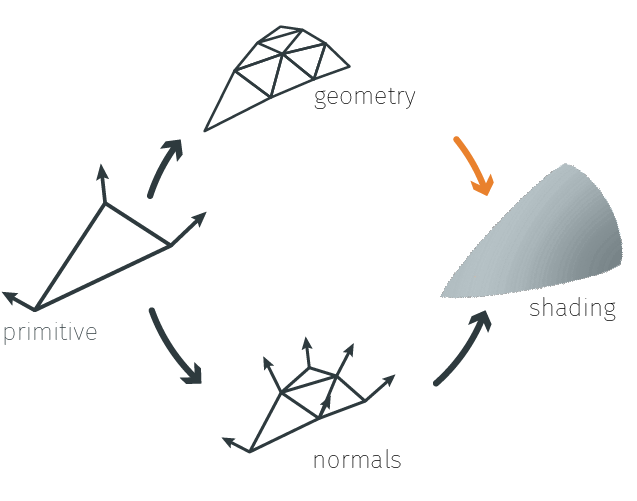
\includegraphics[width=\textwidth]{./img/1_single/recap_inputToNormals.png}
			\end{center}		
		\end{column}
	\end{columns}
	\note<1>{\textbf{[Rick]} From the primitive normals the the PN triangle normals}
\end{frame}	

\begin{frame}\frametitle{Normals}
\enhancement{emphasize normals more}
	\begin{columns}
		\begin{column}{0.6\textwidth}
			\begin{center}
				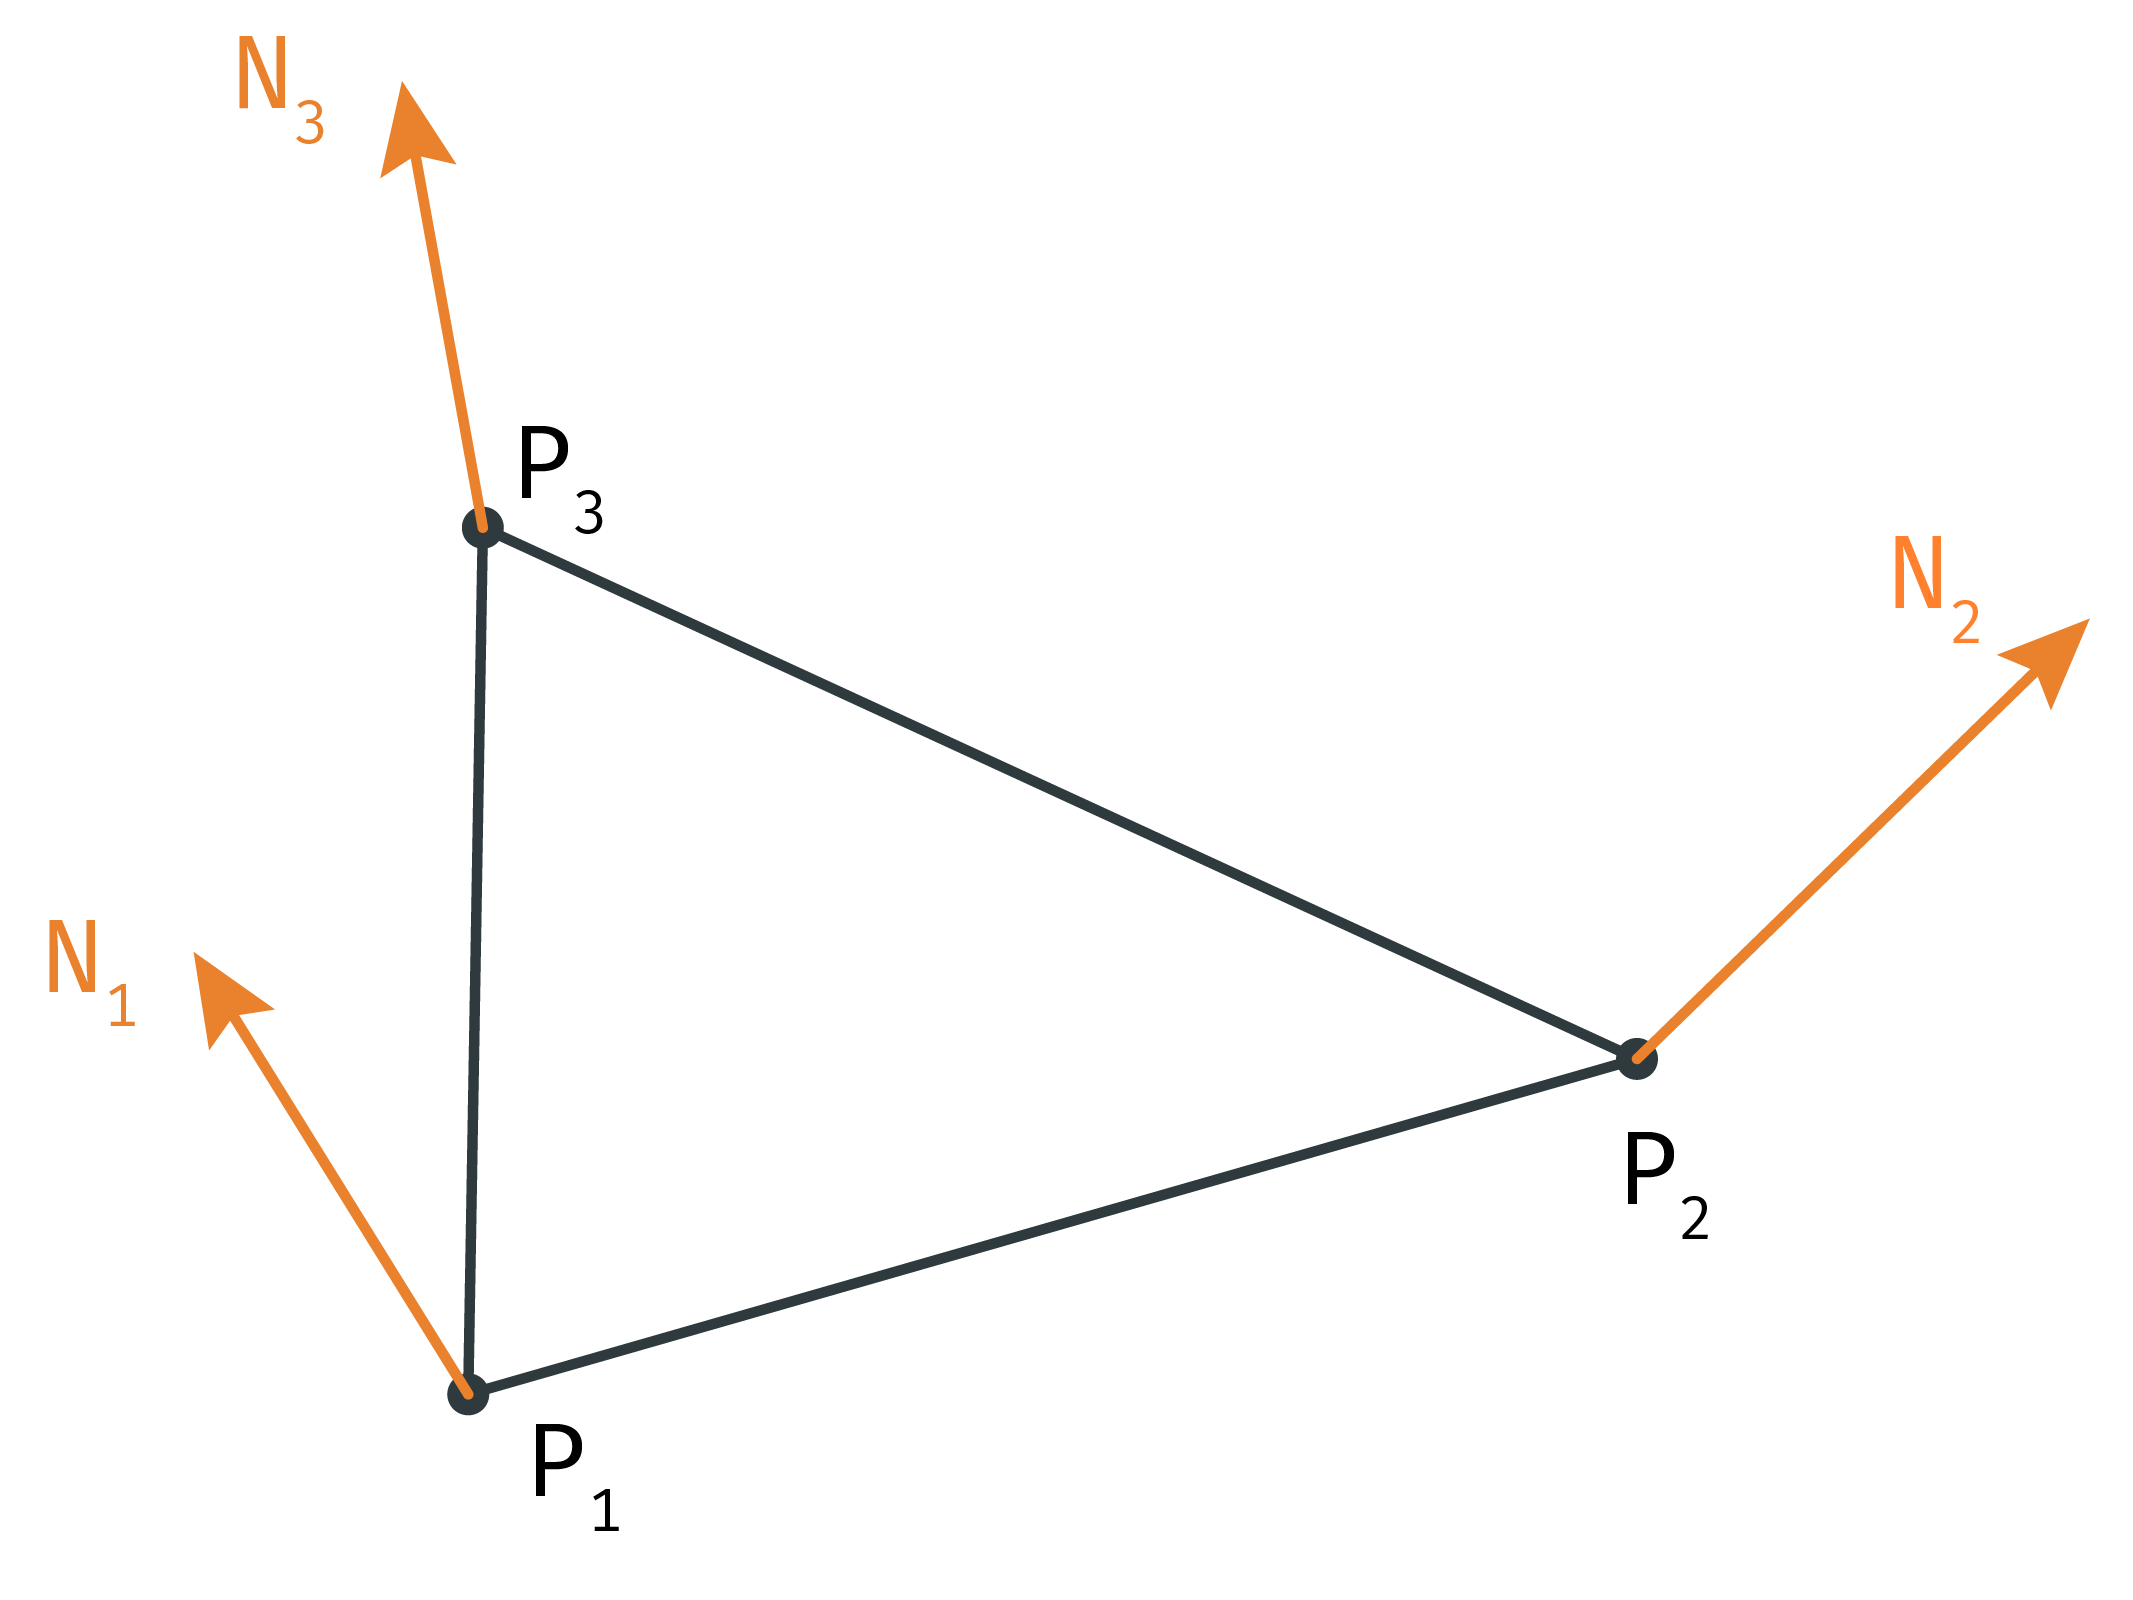
\includegraphics[width=\textwidth]{img/1_single/inputPrimitive_emphNormal.png}
				\small{input primitive}
			\end{center}
		\end{column}
	\end{columns}
	\note<1>{\textbf{[Rick]} Recap input primitive and with emphasis on the normals.}
\end{frame}

\begin{frame}\frametitle{Normals - theory}
	\begin{columns}
		\begin{column}{0.6\textwidth}
			\begin{center}
				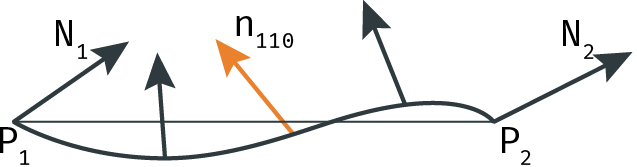
\includegraphics[width=\textwidth]{img/1_single/linearVsQuadraticNormals_linear.png}
				\small{linear}
			\end{center}	
		\end{column}
	\end{columns}
	\pause
	\vspace{0.8cm}
	\begin{columns}
		\begin{column}{0.6\textwidth}
			\begin{center}
				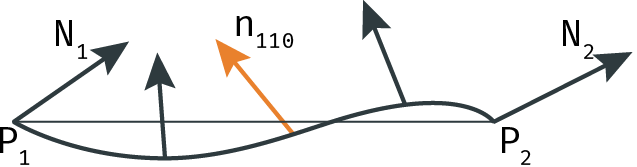
\includegraphics[width=\textwidth]{img/1_single/linearVsQuadraticNormals_quadratic.png}
				\small{quadratic}
			\end{center}	
		\end{column}
	\end{columns}
	\note<1>{\textbf{[Rick]} Stress that there is a need to capture the cubic bezier curve (inflection points) and that this cannot be }
	\note<2>{\textbf{[Rick]} Quadratic does capture inflection points. Trade off between performance and result (maybe?)}
\end{frame}

\begin{frame}\frametitle{Normals - example}
	\begin{columns}
		\begin{column}{0.4\textwidth}
		\begin{center}
				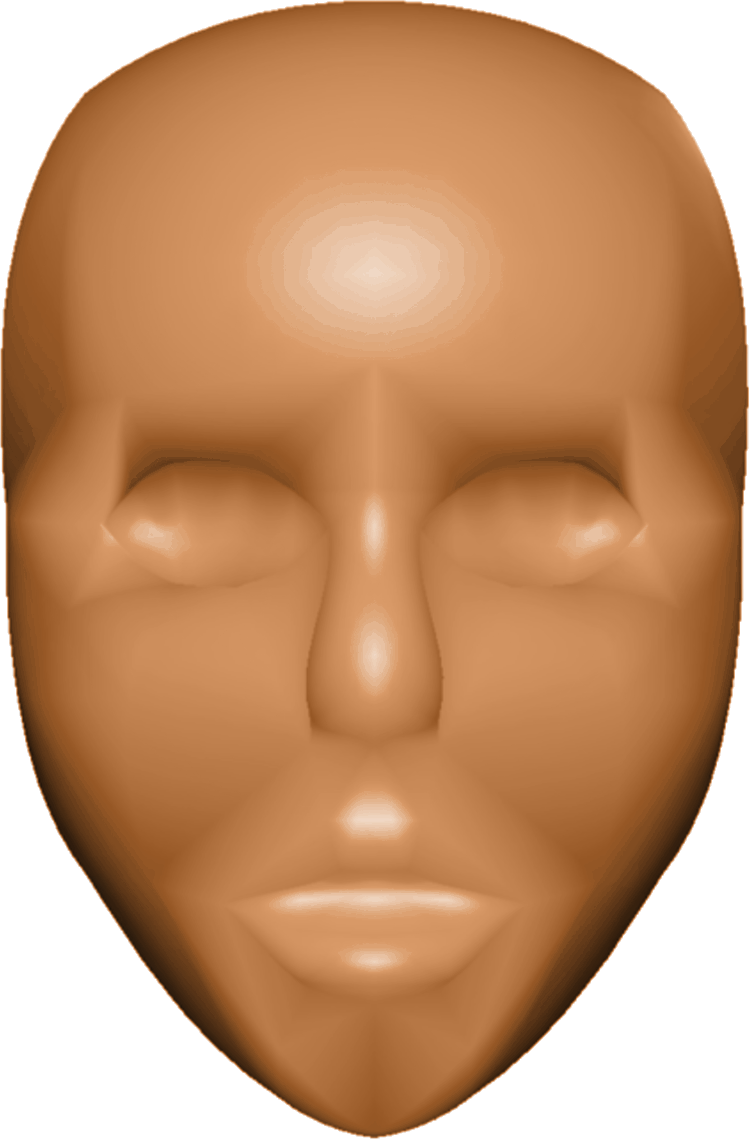
\includegraphics[width=\textwidth]{img/1_single/linearlyVaryingNormals.png}
				\small{linear}
			\end{center}	
		\end{column}
		\begin{column}{0.4\textwidth}
		\begin{center}
				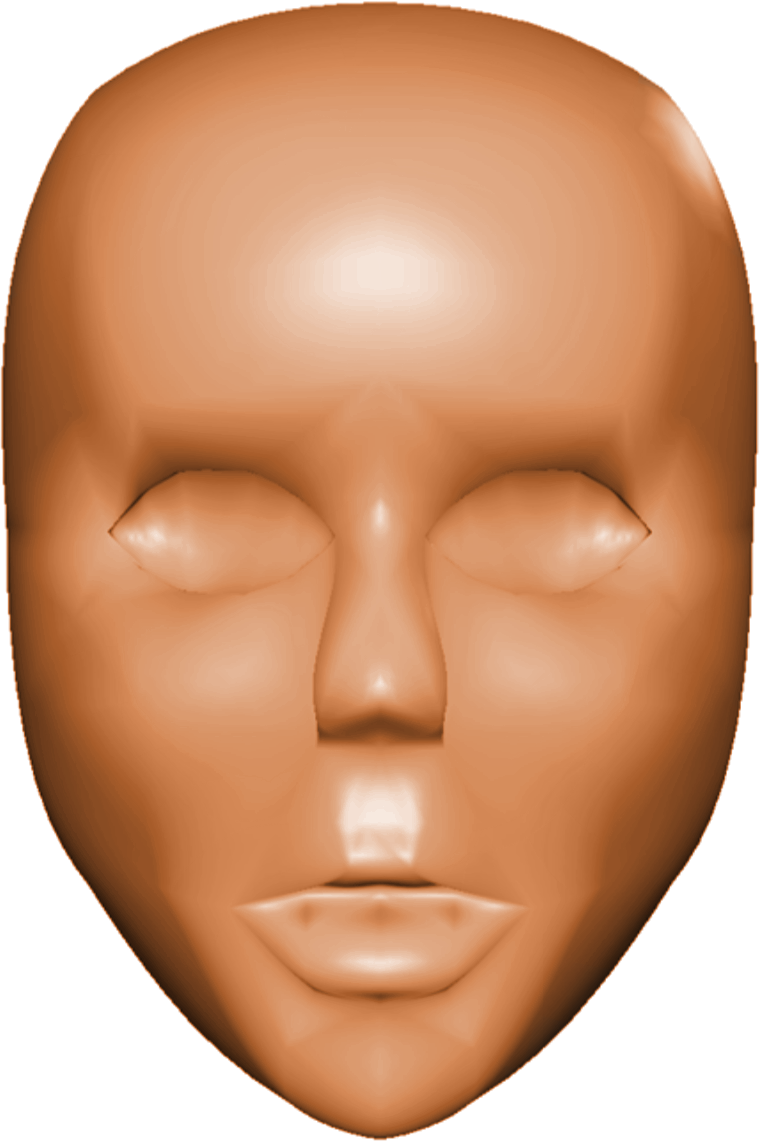
\includegraphics[width=\textwidth]{img/1_single/quadriticallyVaryingNormals.png}
				\small{quadratic}
			\end{center}	
		\end{column}
	\end{columns}
	\note<1>{\textbf{[Rick]} Look how pretty.}
\end{frame}


\begin{frame}\frametitle{Normals - theory}
	\begin{columns}
		\begin{column}{0.6\textwidth}
			\begin{center}
				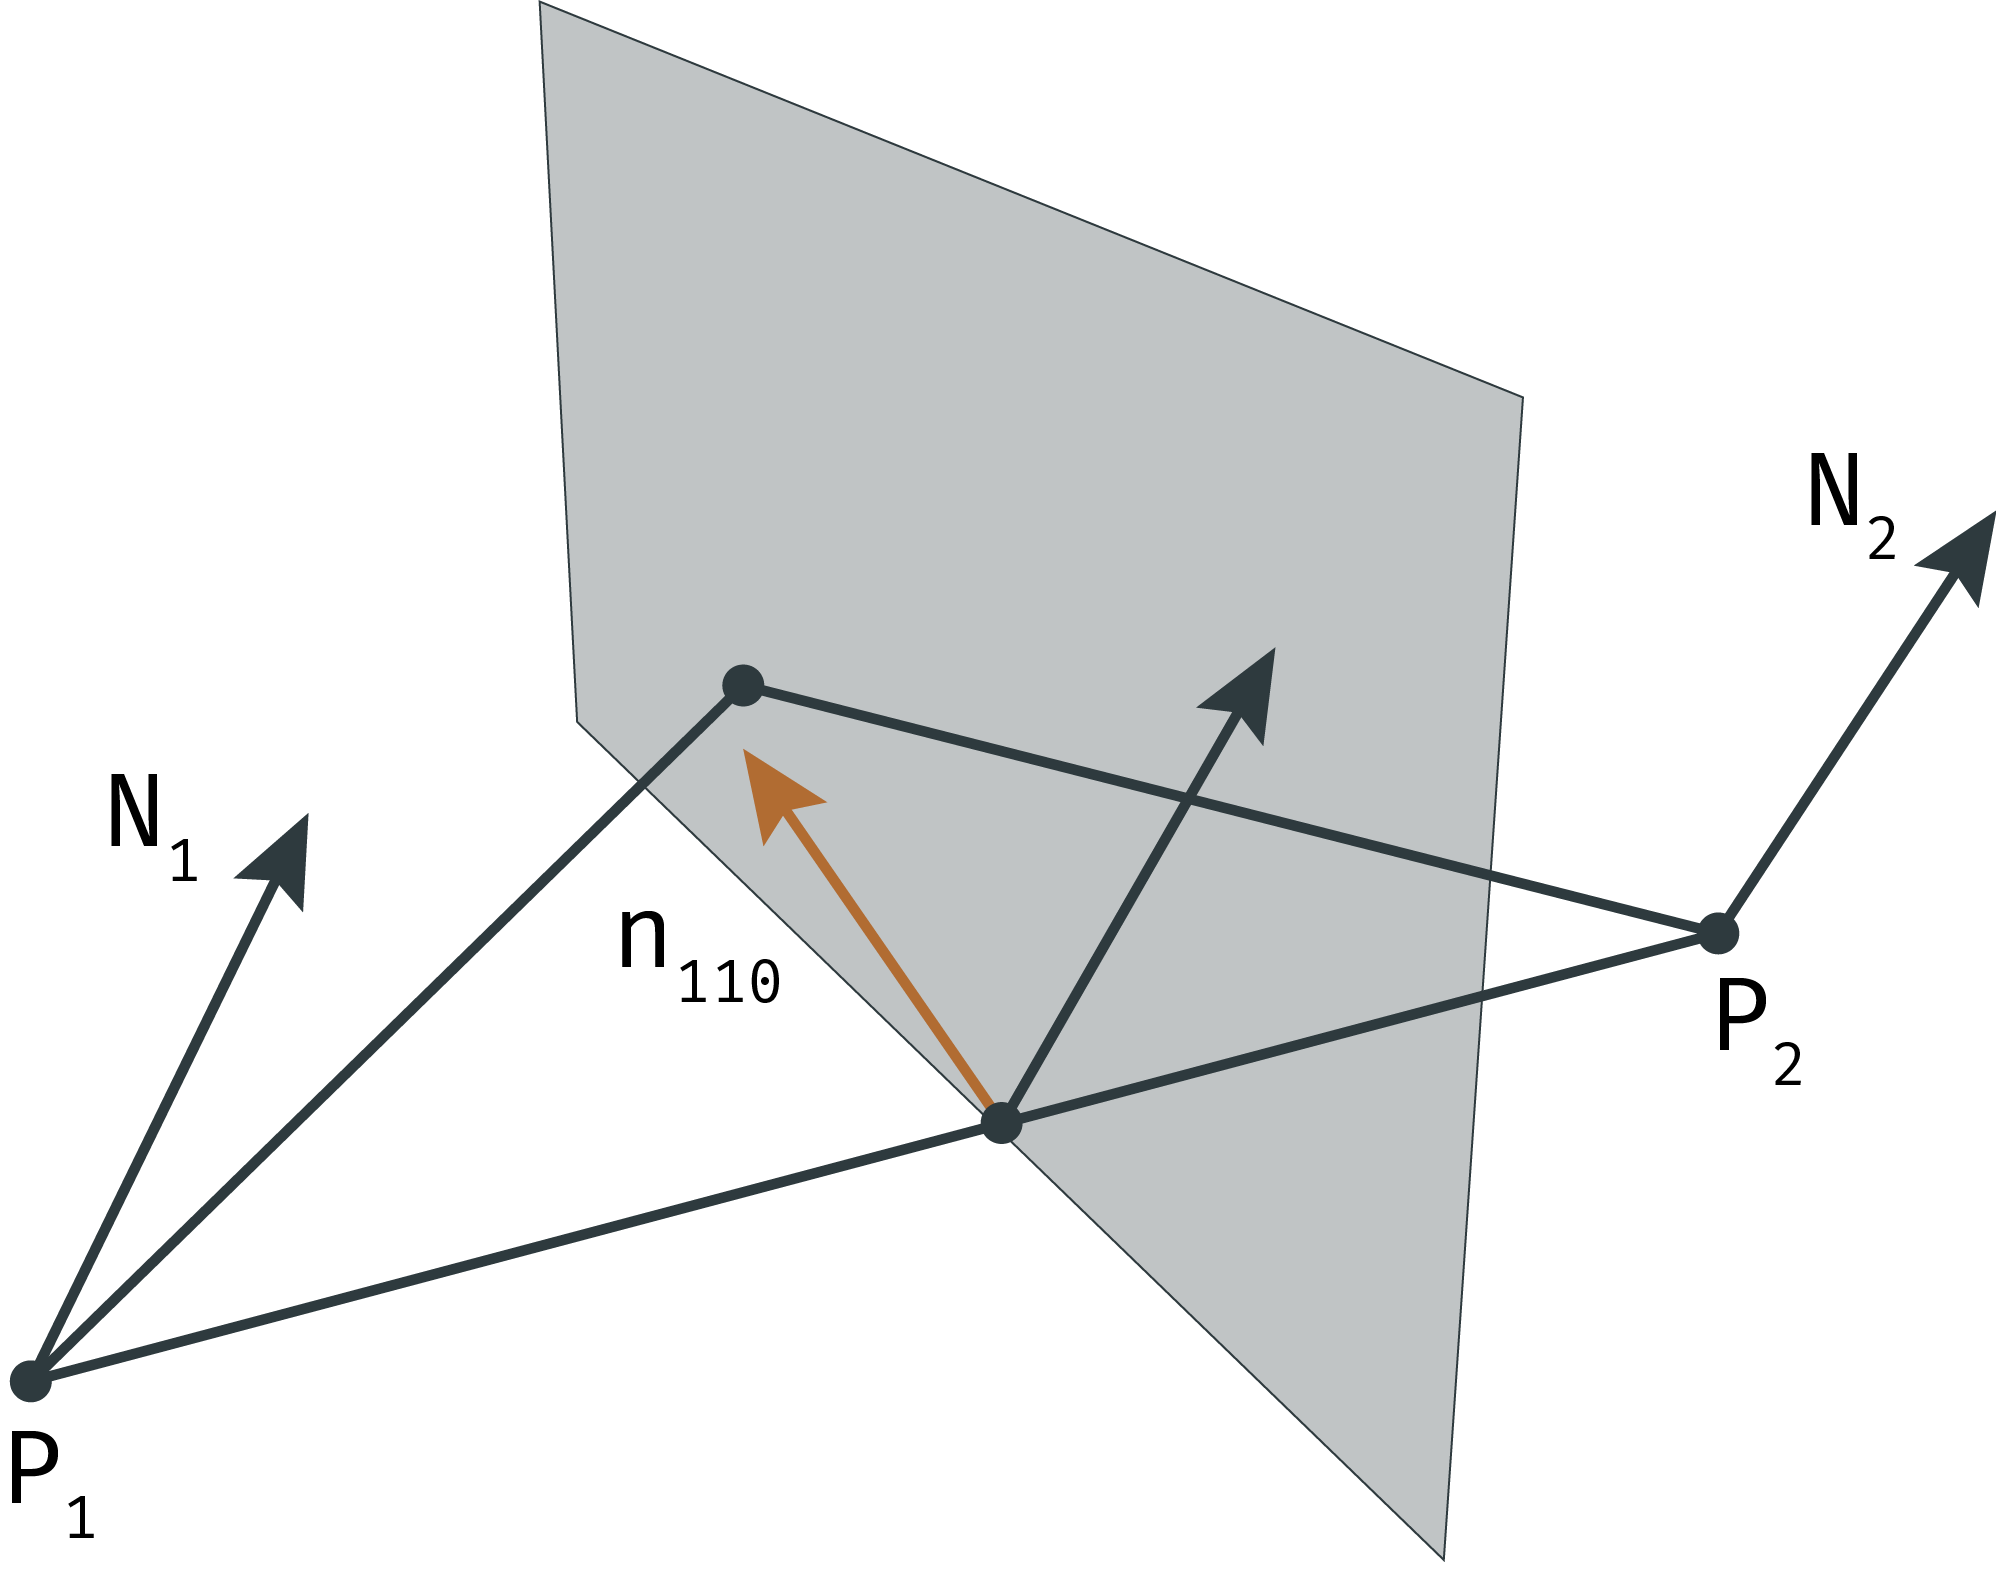
\includegraphics[width=\textwidth]{img/1_single/computingNormals.png}
			\end{center}
		\end{column}
	\end{columns}
	
	\begin{columns}
		\begin{column}{0.4\textwidth}
			\uncover<2>{
				\begin{equation*}
				\begin{aligned}
					v_{ij}  & = 2\frac{(P_j - P_i) \cdot (N_i + N_j)}{(P_j - P_i) \cdot (P_j - P_i)} \in \mathbb{R} \\
					h_{110} & = N_1 + N2 - v_{12}(P_2 - P_1)\\
					n_{110} & =	h_{110} / ||h_{110}||
				\end{aligned}
				\end{equation*}
			}
		\end{column}
	\end{columns}
	\note{\textbf{[Rick]} Formula in words: reflect the averaged normal (average of N1 and N2) on the plane orthogonal/perpendicular the the edge at the mid point.}
\end{frame}

\begin{frame}
	\frametitle{Normals - result}
	\enhancement{Set result slide to plain}
	\begin{columns}
		\begin{column}{0.6\textwidth}
			\begin{center}
				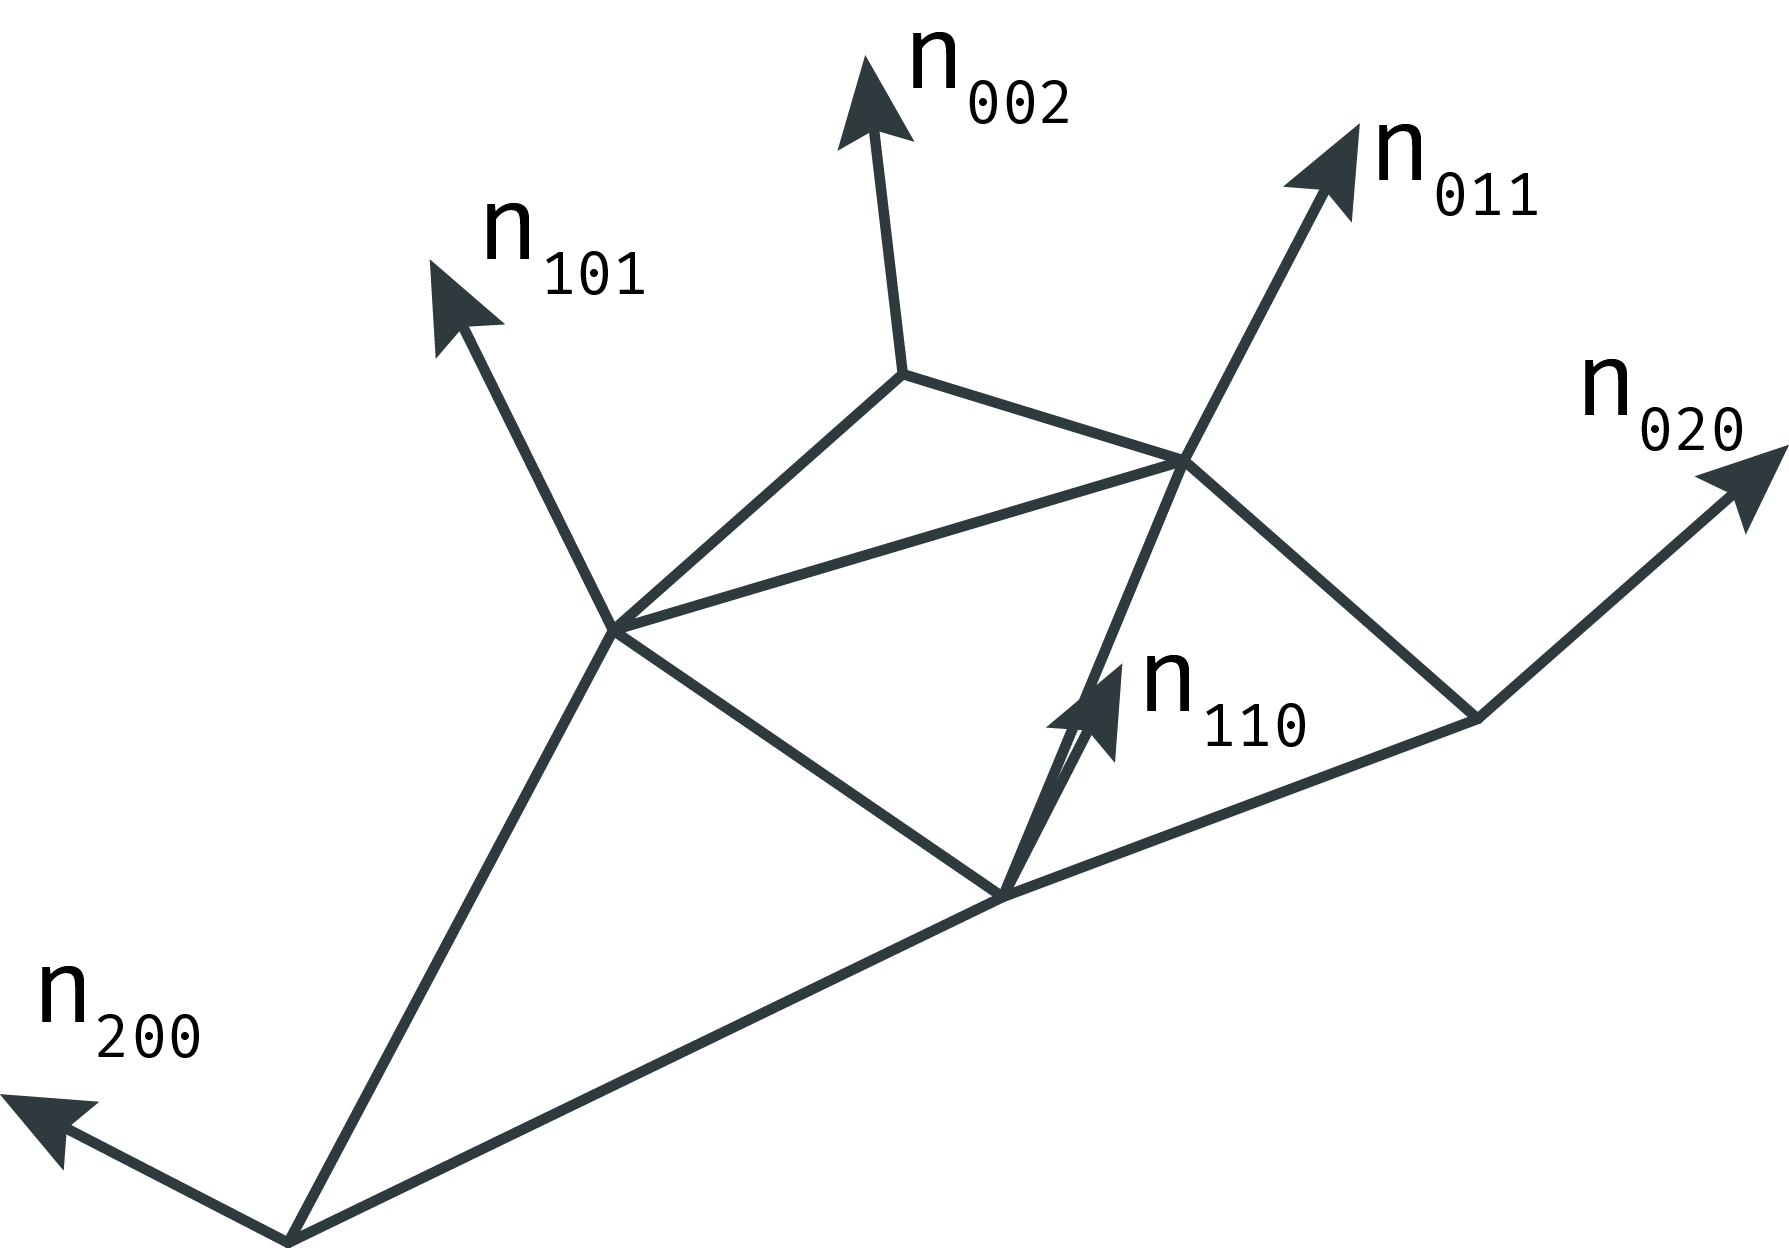
\includegraphics[width=\textwidth]{img/1_single/normals.png}
			\end{center}	
		\end{column}
	\end{columns}
	\note<1>{\textbf{[Rick]} Result}
\end{frame}

\begin{frame}\frametitle{Overview}
	% \todo[inline]{The steps. Recap of everything construct geometry and normals and evaluate less (low lod) or more points (high lod)}
	\begin{columns}
		\begin{column}{0.9\textwidth}
			\begin{center}
				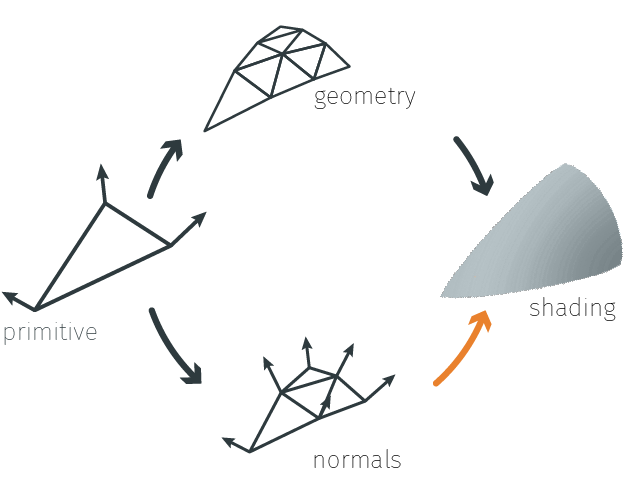
\includegraphics[width=\textwidth]{./img/1_single/recap_normalsToShading.png}
			\end{center}		
		\end{column}
	\end{columns}
	\note{\textbf{laura}}
\end{frame}

\begin{frame}
	\frametitle{Quadratic Patch}
	\begin{columns}
		\begin{column}{0.5\textwidth}
			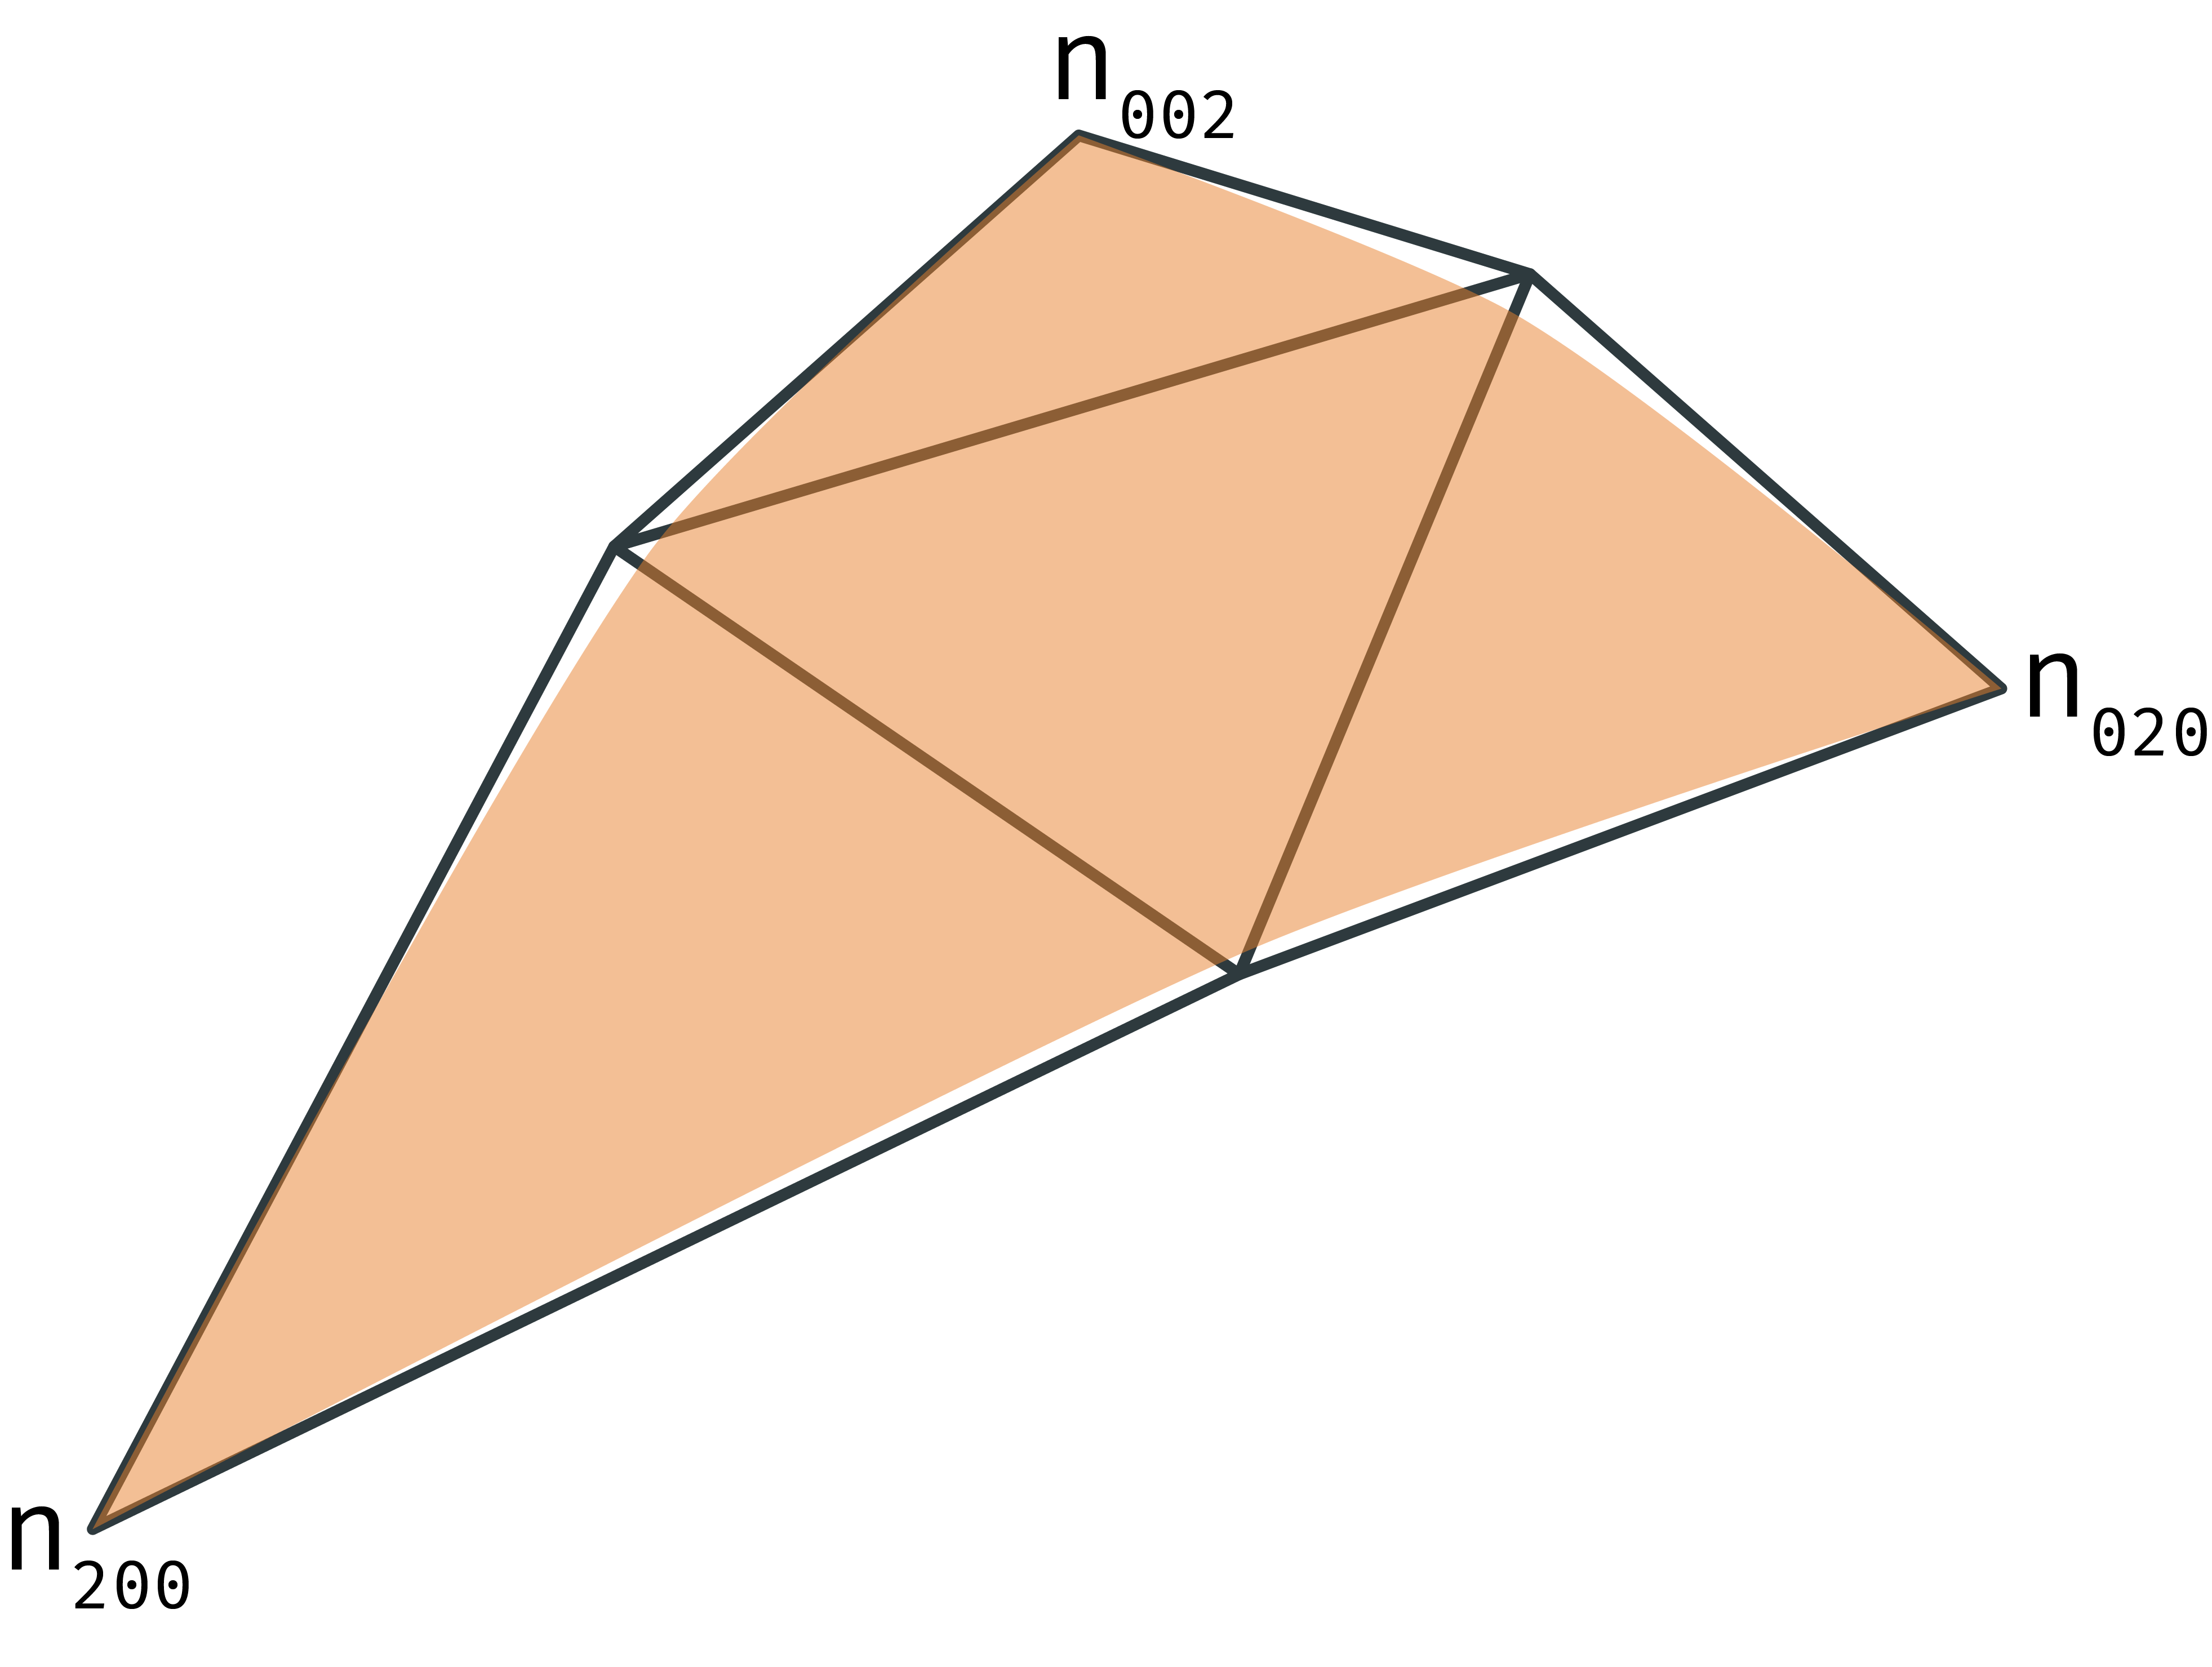
\includegraphics[width=\textwidth]{img/1_single/quadraticPatch.png}
		\end{column}
		\begin{column}{0.5\textwidth}
			\begin{equation*}
				w = 1 - u - v
			\end{equation*}
			\begin{equation*}
				u,\, v,\, w \geq 0
			\end{equation*}
			\begin{equation*}
				n(u,v) = \sum\limits_{i+j+k=2} n_{ijk} u^i v^j w^k
			\end{equation*}
		\end{column}		
	\end{columns}
	\note<1>{\textbf{[Laura]} u, v and w are an convex combination}
\end{frame}